\subsection{Sequence Diagram}
\begin{figure}[h]
\caption{Sequence diagram to retrieve a list of players and roles}
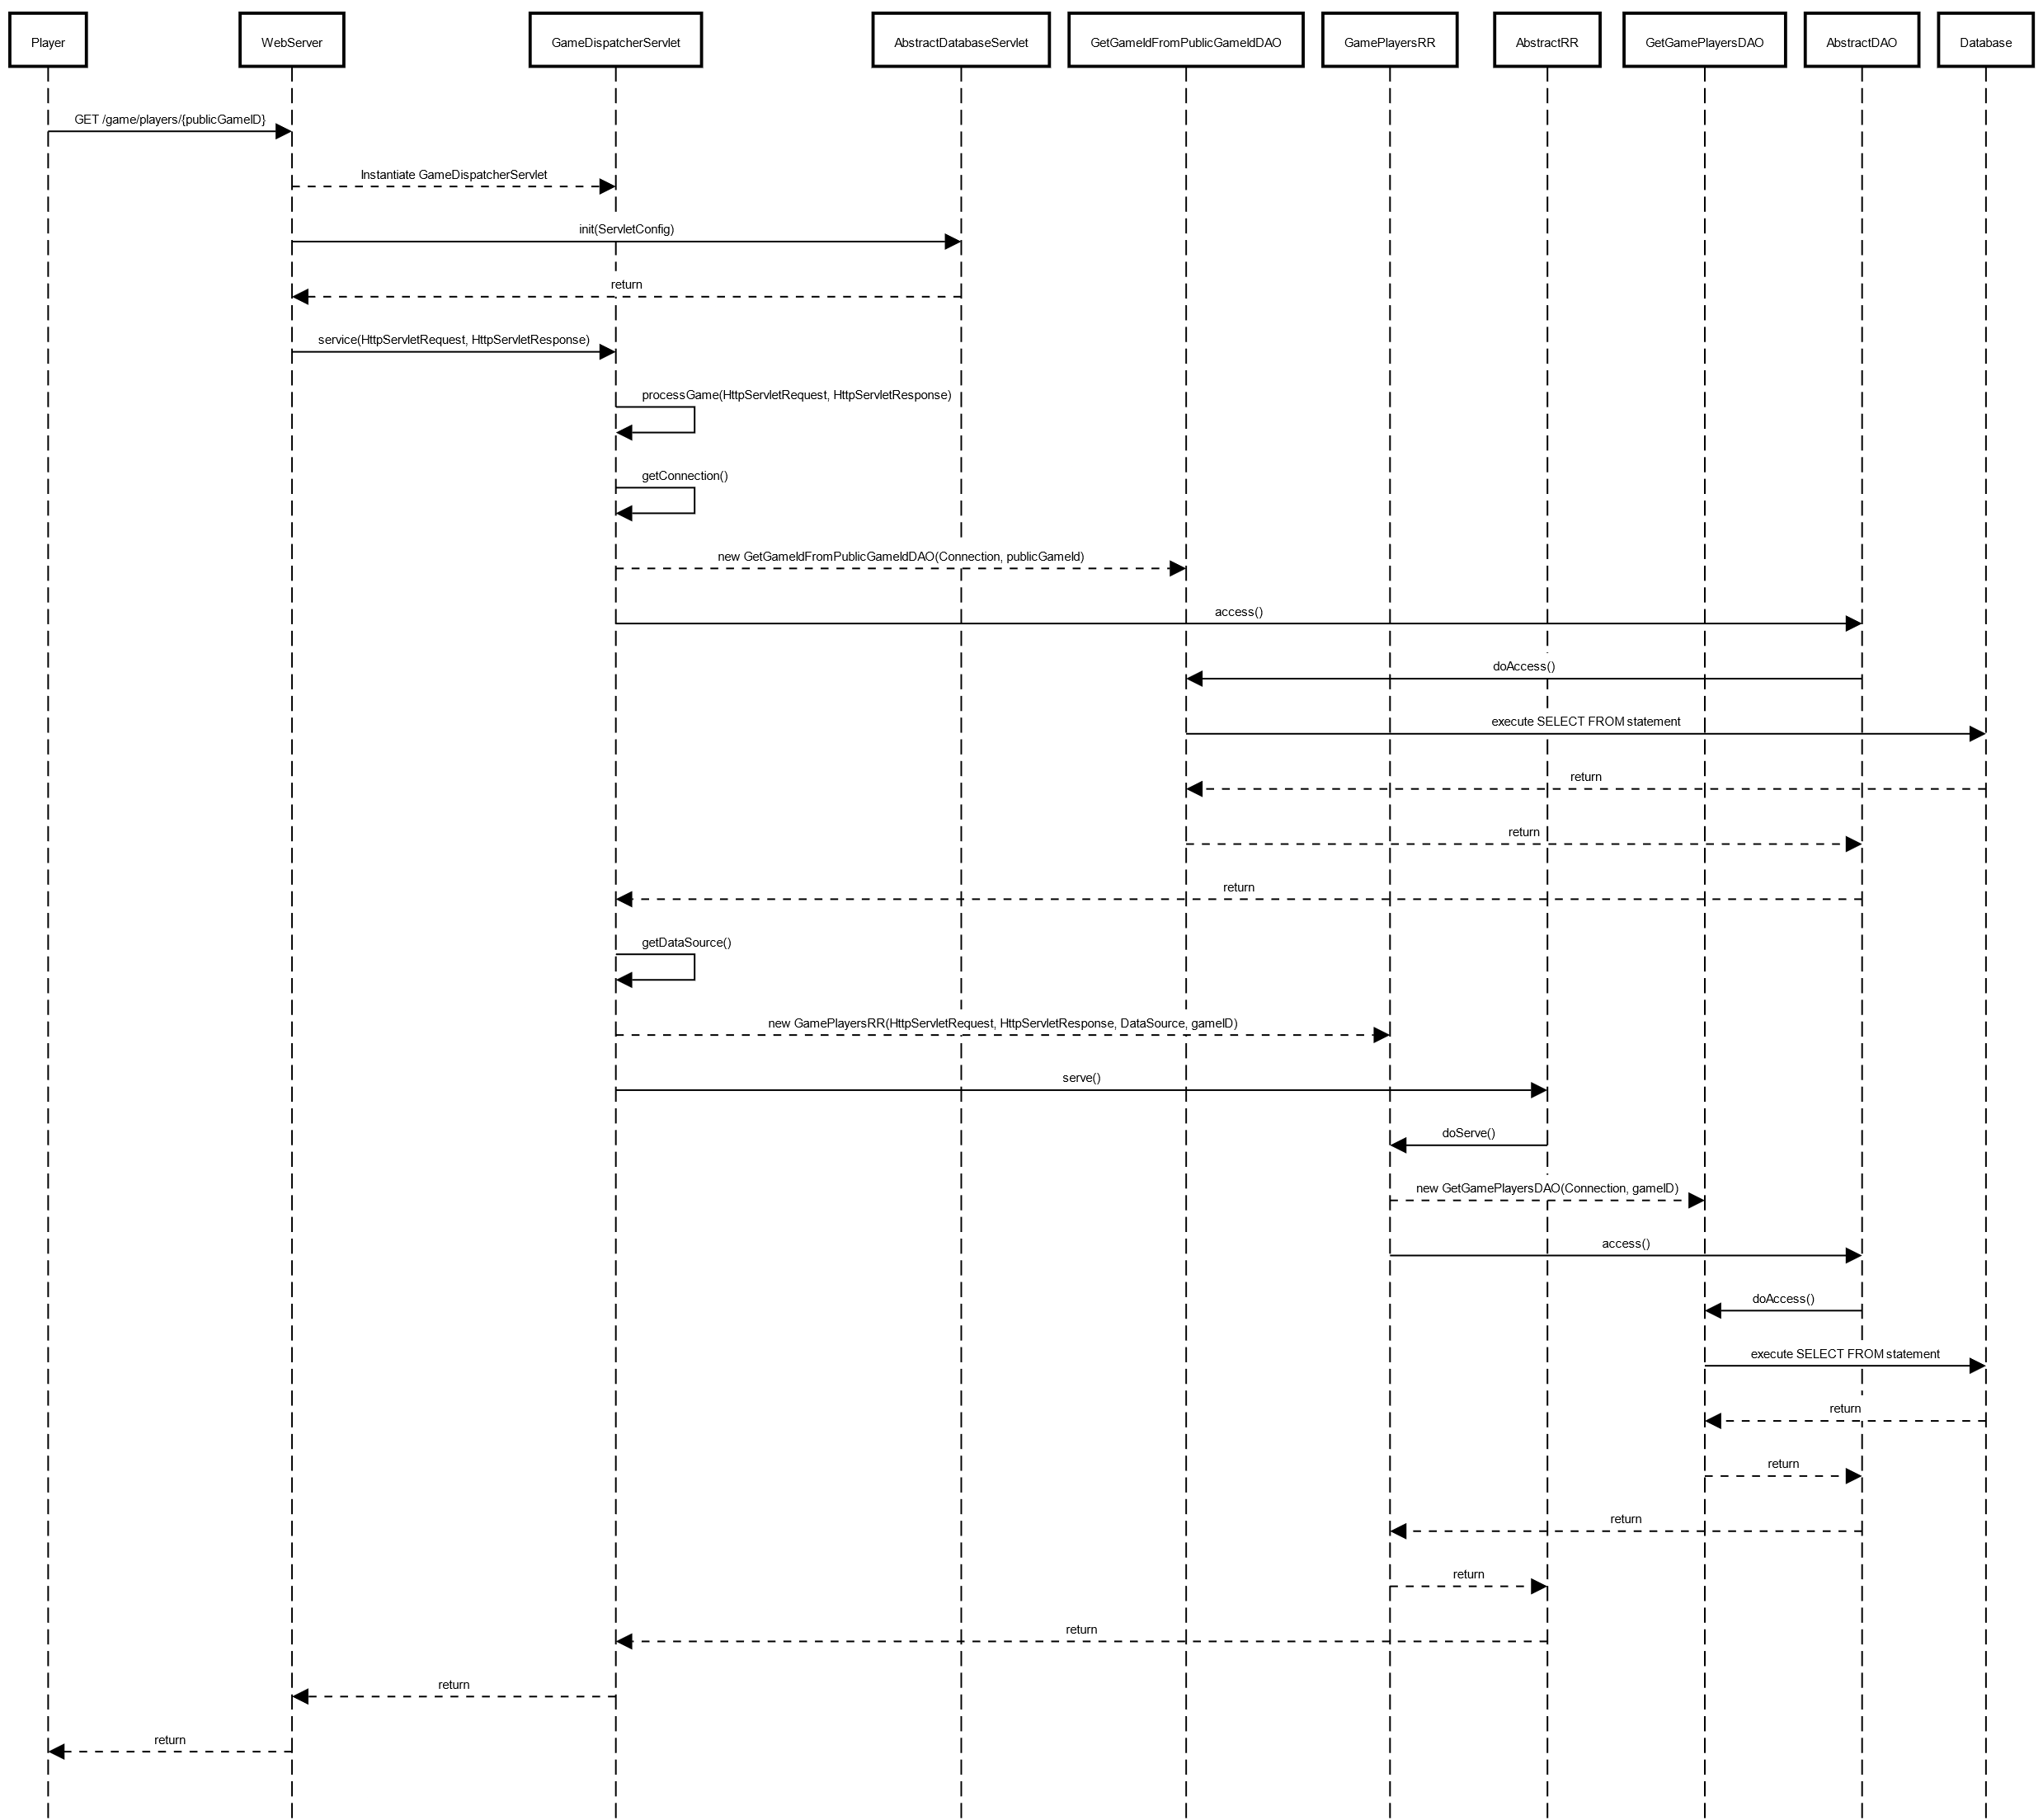
\includegraphics[scale=0.2]{images/seq_dia.png}
\end{figure}

%describe here the sequence diagram
Here we report the sequence diagram to retrieve the list of players and roles that are playing a match identified by a public game ID. The player issues a GET request to the web server at the following URI: /game/players/\{publicGameId\}. The web server instantiates the GameDispatcherServlet which calls its processGame() method, passing the HttpServletRequest and HttpServletResponse. \\
Firstly, the control is passed to the GetGameIdFromPublicGameIdDAO which receives as arguments the connection (defined in the AbstractDatabaseServlet extended by the GameDispatcherServlet) and the publicGameID taken from the URI. The GetGameIdFromPublicGameIdDAO extends the AbstractDAO and contacts the Database Server which executes the SQL statement to retrieve the private game ID given the public game ID. If some errors occur, the control is returned to the SessionServlet and a new Message object is created. \\
Then, a rest resource called GamePlayersRR is instantiated. This resource takes in input HttpServletRequest, HttpServletResponse, the data source and the private game ID. This resource proceeds to call GamePlayersDAO which is the DAO that actually returns the list of players and their respective roles. It works similarly to GetGameIdFromPublicGameIdDAO. \\
Finally, the list formatted in JSON is returned to the user.